\documentclass[12pt]{article}
\usepackage[margin=1in]{geometry}
\usepackage[english,russian]{babel}
\usepackage{amsmath,amsthm,amssymb,color,latexsym}
\usepackage{geometry}        
\geometry{letterpaper}    
\usepackage{graphicx}

\newtheorem{problem}{Задача}

\newenvironment{solution}[1][\it{Решение}]{\textbf{#1. } }{$\square$}


\begin{document}
	\noindent Наблюдательная астрофизика\hfill Экзамен\\
	Збродов Владислав 22.С03
	
	\hrulefill
	\section{Блок. Базовые понятия.}
	\subsection{Основные задачи астрофизики и объекты исследований, наблюдательная астрофизика.}
	\textbf{Астрофизика} – раздел астрономии, изучающий физические
	свойства космических объектов и происходящие в них процессы на
	основе общих физических законов.\\
	\\
	\textbf{Что изучает астрофизика:}
	\begin{itemize}
	\item	Строение и эволюция звёзд;
	\item Экзопланеты;
	\item Межзвёздная среда;
	\item Галактика;
	\item Эволюция галактик;
	\item Космология.
	\end{itemize}
	
		\textbf{Основные задачи астрофизики:}
	\begin{itemize}
		\item	Изучение структуры и эволюции звезд:
			\begin{enumerate}
				\item Понимание процессов, происходящих внутри звезд, их жизненного цикла, от рождения до смерти.
				\item Исследование звездных классификаций, спектральных типов и их физических свойств.
			\end{enumerate}
		
		
		\item Исследование галактик:
			\begin{enumerate}
				\item 	Изучение структуры, динамики и эволюции галактик.
				\item 	Исследование активных галактических ядер и квазаров.
				\item 	Понимание процессов звездообразования и взаимодействия галактик.
			\end{enumerate}
		\item Космология:
			\begin{enumerate}
				\item 	Изучение происхождения, структуры и эволюции Вселенной.
				\item 	Исследование темной материи и темной энергии.
				
				\item 	Понимание космического микроволнового фона.
			\end{enumerate}
		\item Планетарные системы:
			\begin{enumerate}
				\item 	Изучение состава, структуры и динамики межзвездного газа и пыли.
				\item 	Исследование молекулярных облаков и процессов звездообразования.
			\end{enumerate}
		\item Высокоэнергетические явления:
		\begin{enumerate}
			\item 	Изучение сверхновых, гамма-всплесков, нейтронных звезд и черных дыр.
			\item Исследование космических лучей и высокоэнергетических частиц.
		\end{enumerate}
	\end{itemize}
	Наблюдательная астрофизика играет ключевую роль в понимании Вселенной, предоставляя данные, которые позволяют астрофизикам тестировать и уточнять теоретические модели.
	
	\subsection{Используемые инструменты, методы и источники информации об исследуемых объектах.} 
	\textbf{Наблюдательная астрофизика} использует широкий спектр инструментов, методов и источников информации для изучения различных астрономических объектов.
	\textbf{Инструменты наблюдательной астрофизики:}
	\begin{itemize}
		\item \textbf{Оптические телескопы:}
				\begin{enumerate}
				\item 	\textbf{Наземные телескопы}: Большие оптические телескопы, такие как Keck, VLT (Very Large Telescope), и Subaru, используются для наблюдений в видимом и ближнем инфракрасном диапазонах.
				\item \textbf{Космические телескопы}: Хаббл (Hubble Space Telescope) и Джеймс Уэбб (James Webb Space Telescope) предоставляют высококачественные изображения и спектры без атмосферных помех.
			\end{enumerate}
		\item\textbf{Радиотелескопы}:	
				\begin{enumerate}
				\item 	\textbf{Наземные радиотелескопы}: ALMA (Atacama Large Millimeter/submillimeter Array), VLA (Very Large Array), и LOFAR (Low-Frequency Array) используются для наблюдений в радиодиапазоне.
				\item \textbf{Космические радиотелескопы}: Радиотелескопы на орбите, такие как Spektr-R, позволяют избежать атмосферных помех.
			\end{enumerate}
			
			\item\textbf{Инфракрасные телескопы}:	
		\begin{enumerate}
			\item 	\textbf{Наземные инфракрасные телескопы}: IRTF (Infrared Telescope Facility) и UKIRT (United Kingdom Infrared Telescope).
			\item \textbf{Космические инфракрасные телескопы}: Spitzer Space Telescope и Herschel Space Observatory.
		\end{enumerate}	
		
		
			\item\textbf{Ультрафиолетовые телескопы}:	
				\begin{enumerate}
				\item 	\textbf{Космические ультрафиолетовые телескопы}: GALEX (Galaxy Evolution Explorer) и Swift.
			\end{enumerate}	
			
		\item\textbf{Рентгеновские телескопы}:	
		\begin{enumerate}
			\item 	\textbf{Космические рентгеновские телескопы}:Chandra X-ray Observatory и XMM-Newton.
		\end{enumerate}	
		
		\item\textbf{Гамма-телескопы}:	
		\begin{enumerate}
			\item 	\textbf{Космические гамма-телескопы}: Fermi Gamma-ray Space Telescope.
				\item 	\textbf{Наземные гамма-телескопы}: Cherenkov Telescope Array (CTA) и HESS (High Energy Stereoscopic System).
		\end{enumerate}		
	\end{itemize} 
	
		\textbf{Методы наблюдательной астрофизики:}
	\begin{itemize}
		\item \textbf{Фотометрия:}
		\begin{enumerate}
			\item Измерение яркости небесных объектов в различных диапазонах спектра.
			\item Используется для определения светимости, температуры и расстояния до объектов.
		\end{enumerate}
		\item\textbf{Спектроскопия}:	
		\begin{enumerate}
			\item Анализ спектров небесных объектов для определения их состава, температуры, скорости и других физических параметров.
			\item Используется для изучения химического состава звезд, галактик и межзвездной среды.
		\end{enumerate}
		
		\item\textbf{Интерферометрия}:	
		\begin{enumerate}
			\item Использование нескольких телескопов для создания виртуального телескопа с высоким разрешением.
			\item Применяется в радиоастрономии (VLBI) и оптической астрономии (VLTI).
		\end{enumerate}	
		
		
		\item\textbf{Поляриметрия}:	
		\begin{enumerate}
			\item 	Измерение поляризации света от небесных объектов.
			\item Используется для изучения магнитных полей и структуры межзвездной среды.
		\end{enumerate}
	\end{itemize}
	Приёмники излучения используются для обнаружения и анализа ЭМ излучения от объектов. В зависимости от диапазона спектра, применяются различные типы приёмников.\\
	\textbf{Источники информации об исследуемых объектах:}
	\begin{itemize}
		\item Электромагнитное излучение;
		\item Нейтрино;
		\item Гравитационные волны;
		\item Космические лучи.
	\end{itemize}
	
	
	
	\subsection{Электромагнитное излучение, основные характеристики и единицы измерений.}
	
	Основным источником информации о небесных телах остаётся ЭМ излучение.
	Спектральный состав характеризуется длиной волны
	излучения $\lambda$ или частотой $\nu$.
	
	\begin{center}
		\begin{tabular}{||c c c||} 
			\hline
			Диапазон & Энергия($h\nu$) &Температура ($h\nu/k$) \\ [0.5ex] 
			\hline\hline
			Гамма лучи & $10^5$ эВ& $10^9$ К  \\ 
			\hline
			X & $10^3$ эВ& $10^7$ К  \\
			\hline
			УФ & $10$ эВ& $10^5$ К  \\
			\hline
			Видимый & $1$ эВ& $10^4$ К  \\
			\hline
			ИК & $0.1$ эВ& $10^3$ К   \\
			\hline
			Микроволновый & $10^{-3}$ эВ& $10$ К   \\
			\hline
			Радио & $10^{-6}$ эВ& $0.001$ К   \\
			\hline
		\end{tabular}
	\end{center}
	\textbf{dQ} -- энергия от источника.
	\textbf{Поток излучения - энергия, протекающая через площадку $dA$ за время $dt$.}
	$$F = \frac{dQ}{dt}$$ 	Измеряется в эрг/с или других единицах мощности, например в
	ваттах.
\begin{figure}[h]
	\centering
	\includegraphics[width=0.3\linewidth]{"111"}
\end{figure}\\
	Освещенность или плотность потока -- пото с единичной площадки $dS$:
	$$E = \frac{dF}{dS}$$ Измеряется в эрг/с/см$^2$\\
	\textbf{Интенсивность точечного источника}
	$$I = \frac{dF}{d\Omega}$$
	$$d\Omega = \frac{dS}{r^2}$$
	Характеризует излучательные свойства источника, и не зависит от того, на каком расстоянии от него поместить элементарную площадку.	\\
	\textbf{Поверхностная яркость протяженного источника:}
	$$B = \frac{I}{\sigma}$$
	$\sigma$ -- проекция площадки на плоскость, перпендикулярную направлению распространения света, измеряется в эрг/с/стерад/см$^2$\\
	Удельная плотность потока измеряется в ватт/м$^2$/Гц, Янский (1 Ян $= 10^{-26}$ ватт/м$^2$/Гц)\\
	Переход от $\nu$ к $\lambda$:
	$$\lambda E_{\lambda}= \nu E_{\nu}$$
	\textbf{Пример}:
	Удельная освещенность на $10^8$ Гц ($\lambda = 300$ см)
	составляет $E_{\nu}	= 17\cdot10^{-23}$ вт/м$^2$/Гц.
	\subsection{Земная атмосфера, её влияние, условия наблюдений, внеатмосферные источники искажений.}
	Земная атмосфера оказывает значительное влияние на наблюдения в астрономии, как в оптическом, так и в других диапазонах электромагнитного спектра. \\
	\textbf{Земная атмосфера:}
	\begin{itemize}
		\item Поглощение и рассеяние света:
			\begin{enumerate}
				\item \textbf{Поглощение}: Молекулы и аэрозоли в атмосфере поглощают свет определенных длин волн, что приводит к ослаблению сигнала от астрономических объектов. Например, озон в атмосфере поглощает ультрафиолетовое излучение, а водяной пар поглощает инфракрасное излучение.
				\item \textbf{Рассеяние}: Рассеяние света на молекулах и частицах в атмосфере (так называемое рассеяние Рэлея) приводит к уменьшению яркости объектов и ухудшению контраста изображений.
			\end{enumerate}
			\begin{figure}[h]
				\centering
				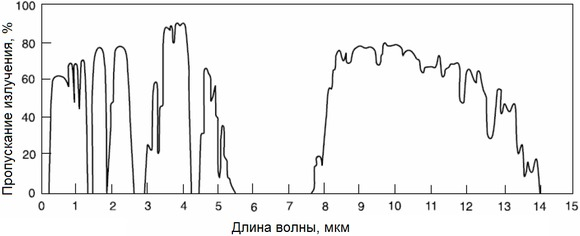
\includegraphics[width=0.7\linewidth]{atmosphere}
			\end{figure}
			Рассеяние света: на молекулах воздуха, коэффициент рассеяния пропорционален $\sim \lambda^{-4}$,
		на аэрозоле коэффициент пропорционален $ \sim \lambda^{-\alpha} $, где $ \alpha \approx 0.8$;
		\item \textbf{Атмосферная помутненность}: Турбулентность в атмосфере вызывает колебания плотности воздуха, что приводит к искажению волнового фронта света, проходящего через атмосферу. Это явление называется атмосферной помутненностью и ограничивает угловое разрешение наземных телескопов.
		
		\item \textbf{Атмосферная дисперсия}: Различные длины волн света преломляются в атмосфере по-разному, что приводит к хроматической аберрации и искажению изображений.
	\end{itemize}

	\textbf{Условия наблюдений:}
	\begin{itemize}
		\item \textbf{Высокогорные обсерватории}: Расположение обсерваторий на высоких горах (например, Мауна-Кеа на Гавайях) снижает влияние атмосферы, так как количество атмосферы над телескопом уменьшается.
		\item \textbf{Сухие и стабильные климатические условия}: Обсерватории часто строятся в пустынных или полупустынных районах с низкой влажностью и стабильной погодой, что снижает влияние водяного пара и атмосферной турбулентности.
	\end{itemize}
	
	\textbf{Внеатмосферные источники искажений:}
	\begin{itemize}
		\item \textbf{Космические лучи}: Высокоэнергетические частицы, попадающие в атмосферу Земли, могут создавать фоновый шум и искажения в детекторах.
		\item \textbf{Солнечный свет}: Рассеянный солнечный свет может создавать фоновый шум, особенно при наблюдениях в дневное время или в сумеречное время.
		\item \textbf{Ионосфера}: Ионосфера Земли может искажать радиосигналы, особенно на низких частотах.
	\end{itemize}
	
	\textbf{Способы избежать влияния атмосферы:}
	\begin{enumerate}
		\item \textbf{Космические телескопы}: Размещение телескопов на орбите Земли позволяет полностью избежать влияния атмосферы. Примеры космических телескопов включают Хаббл (Hubble Space Telescope) для оптических и ультрафиолетовых наблюдений, Чандра (Chandra X-ray Observatory) для рентгеновских наблюдений и Спитцер (Spitzer Space Telescope) для инфракрасных наблюдений.
		\item \textbf{Баллонные и высотные наблюдения}: Использование воздушных шаров и высотных самолетов позволяет поднять телескопы на большие высоты, где влияние атмосферы минимально. Примеры включают SOFIA (Stratospheric Observatory for Infrared Astronomy), который размещен на борту самолета.
	\end{enumerate}
	\section{Блок. Оптические телескопы и инструменты.}
	\subsection{Функции телескопа, его основные характеристики и ограничения.}
	Телескоп является основным инструментом в наблюдательной астрофизике, позволяя астрономам собирать свет от далеких объектов и анализировать его для получения информации о Вселенной.\\
		\textbf{Задачи телескопа}: Прием и анализ излучения
		осуществляется с помощью
		телескопа.
	\begin{enumerate}
		\item Собрать и направить на приемник излучения как
		можно большее количество световой энергии;
		\item Отделить положения изображений источников (или
		отдельных деталей) друг от друга;
		\item Выделить сигнал от отдельного источника среди
		естественного шума.
	\end{enumerate}
	\textbf{Функции телескопа}:
	\begin{enumerate}
		\item Увеличение угла зрения (увеличение видимых размеров объекта и разрешения близко расположенных объектов) – по существу приближение объекта.
		\item Увеличение плотности потока (и, тем самым, проницающей силы).
		\item Направление излучения от объекта на приёмник.
	\end{enumerate}
	\textbf{Характеристики телескопа}:
	\begin{enumerate}
		\item Угловое увеличение (Увеличение одиночной линзы).\\
		Равнозрачковое увеличение: $g = D/\delta$, $D$ -- диаметр зеркала, $\delta$ — диаметр зрачка.		
		\item Масштаб изображения -- какой линейный размер в
		фокальной плоскости будет соответствовать угловому
		расстоянию на небе. $L = F \tg{\alpha}$, $\tg{\alpha} \approx \alpha$, $L \approx F \alpha''/ 206265''$
		\item Поле зрения -- угловой размер области неба,
		которую телескоп может качественно отобразить на
		приёмнике излучения.
			\begin{itemize}
				\item Зеркально -- линзовые телескопы системы
				Шмидта и Максутова -- максимальное поле
				зрения $5^{\circ} - 6^{\circ}$
				\item Рефлекторы -- $1^{\circ}$
				\item Визуальные наблюдения -- ограничения окуляра.
				\item Относительное отверстие телескопа -- $A = D/F$ (светосила)
				\item Разрешение -- способность различать
				мелкие детали. (человеческий глаз $\sim1'$)
				\item Теоретическое разрешение $\alpha[rad] = 1.22 \lambda/D$\\
				$a = F\alpha = 1.22 \lambda F/D$ -- линейный радиус кольца.
				\item Разрешающая сила телескопа -- 
				При $\Delta$ между двумя звёздами меньше $2\alpha$
				частичное наложение дифракционных дисков;
				Предел разрешающей силы телескопа:
				$\Delta'' = 0.85 \alpha$
				\item Проницающая сила – способность телескопа
				регистрировать слабые объекты. (Для глаза – $5^{m} - 6^{m}$)
				$$m = 2 + 5\lg D [mm]$$
			\end{itemize}
			
	\end{enumerate}
	\newpage
	
	\subsection{Основные типы телескопов, классические оптические схемы, аберрации оптических систем, потери и ограничения.}
	
	\textbf{Классические схемы}
	
\begin{figure}[h]
	\centering
	\includegraphics[width=0.7\linewidth]{"Снимок экрана от 2024-12-22 17-45-41"}
\end{figure}

Если перед главным фокусом плоское зеркало, то это система Ньютона. Больше поле зрения.
Если вторичное зеркало --выпуклая гипербола, то это Кассегрен. Основное зеркало параболическое. Вторичное зеркало может двигаться – меняется фокусное расстояние;
если совсем убрать вторичное зеркало, то будет схема Ньютона с большим полем зрения.


\begin{figure}[h]
	\centering
	\includegraphics[width=0.4\linewidth]{"Снимок экрана от 2024-12-22 17-45-07"}
\end{figure}

В системе Грегори вторичное зеркало является вогнутым эллипсом.\newpage

\begin{figure}[h]
	\centering
	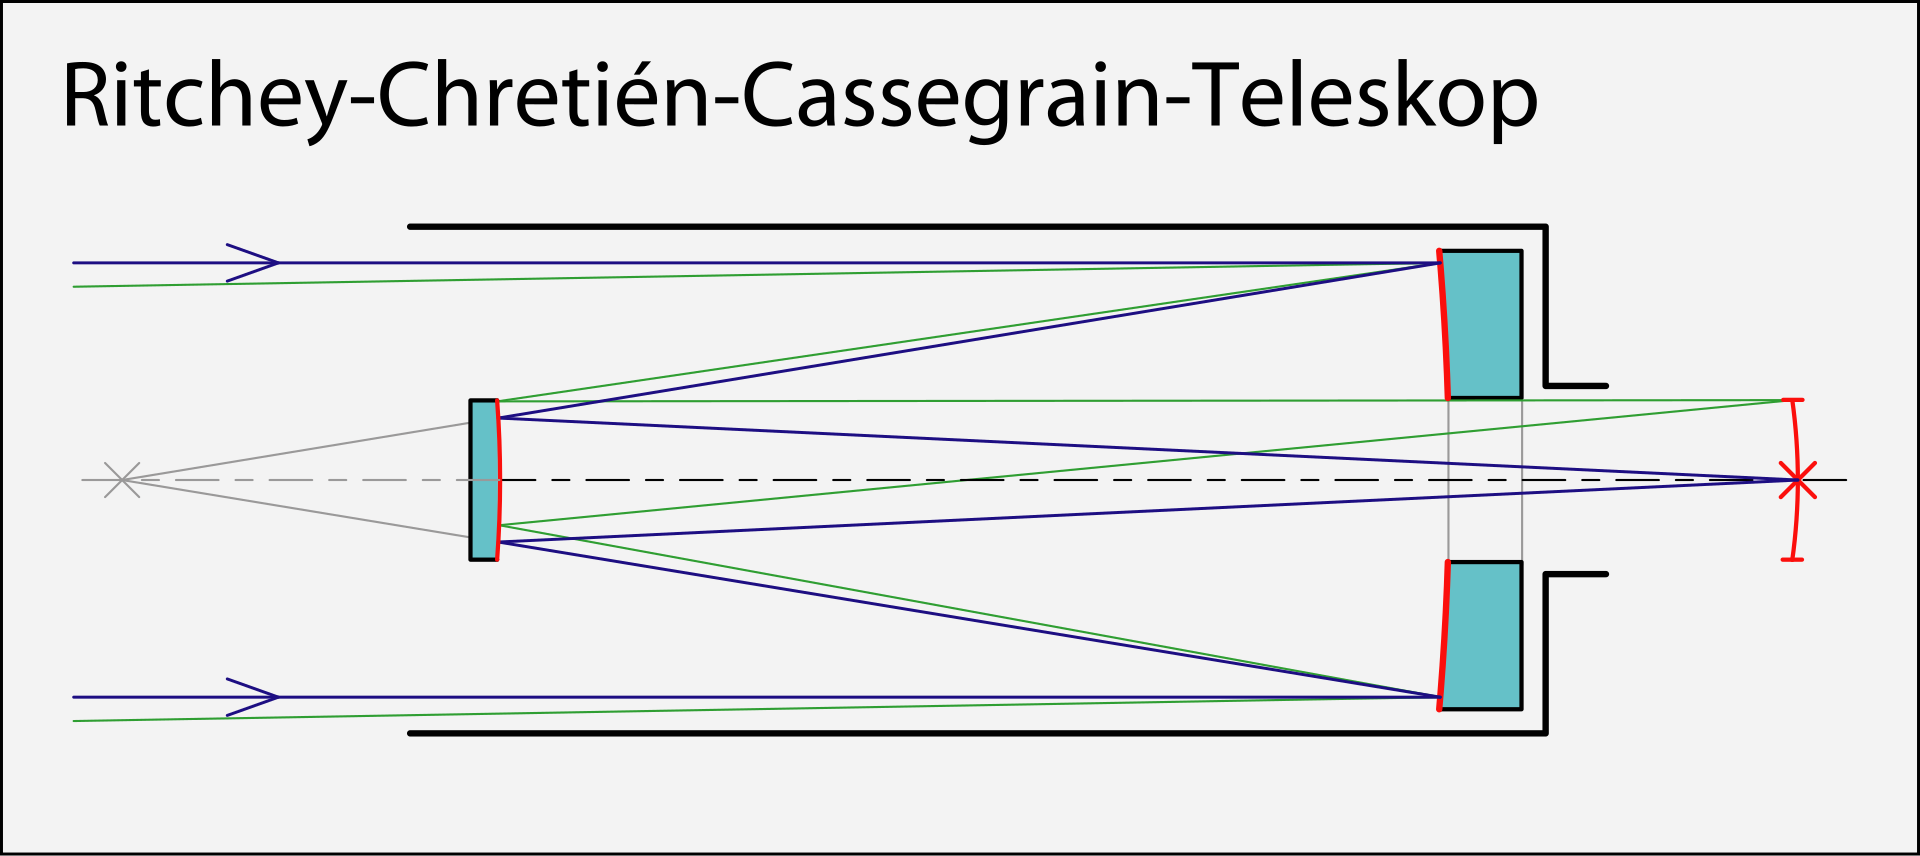
\includegraphics[width=0.7\linewidth]{Ritchey-Chretien-Cassegrain-Teleskop.svg}
\end{figure}
В схеме Ричи--Кретьена оба зеркала (главное вогнутое и
вторичное выпуклое) имеют форму
гиперболоидов вращения. Особенность системы Ричи--Кретьена, отличающая её от большинства других вариантов системы Кассегрена — отсутствие комы третьего порядка и сферической аберрации. С другой стороны, велик высокоугловой астигматизм и кривизна поля; поэтому для получения больших полей применяются
изогнутые пластинки или линзу Пиацци-Смита, которая
устанавливается непосредственно перед фокусом и устраняет
кривизну поля благодаря соответственно подобранной кривизне
самой линзы. Как и прочие кассегрены, имеет короткий корпус, вторичное зеркало, которое в случае системы Ричи--Кретьена является гиперболическим и препятствует появлению комы и способствует широкому полю.\\
\textbf{Пропускание оптики,
	отражение от зеркал.}
\begin{figure}[h]
	\centering
	\includegraphics[width=0.9\linewidth]{"Снимок экрана от 2024-12-22 18-05-30"}
\end{figure}
\newpage
\textbf{Фокус Куде}
\begin{figure}[h]
	\centering
	\includegraphics[width=0.7\linewidth]{"Снимок экрана от 2024-12-22 18-06-40"}
\end{figure}\\
\textbf{Аберрации}\\
Оптическая система должна преобразовать плоский
фронт волны, идущий от бесконечно удалённого объекта,
в сферический, сходящийся в одной точке.
Вносимые искажения называются аберрациями.\\
\textbf{Оптические стекла}
\begin{itemize}
	\item Флинты характеризуются
	малым коэффициентом дисперсии ($\nu_D <
	50$)
	\item Кроны -- большим ($\nu_D > 50)$
	
	Стекла обоих типов называются легкими или
	тяжелыми в зависимости от величины
	показателя преломления.\\
	Обе разновидности стекол имеют общие
	компоненты - $SiO_2$, $Na_2O$, $K_{2}O$.
	Для увеличения $\nu_D$ в состав кронов добавляют
	$B_2O_3$, $Al_2О_3$, $BaO$, $CaO$, а	
	в состав флинтов -- $PbO$, $TiO_2$, $ZnO$, $MgO$, $Sb_2O_3$	
	\begin{figure}[h]
		\centering
		\includegraphics[width=0.5\linewidth]{"Снимок экрана от 2024-12-22 18-23-56"}
	\end{figure}
	
	Исправленные от хроматической аберрации телескопы -- ахроматы,
	апохроматы.
	
\end{itemize}

\begin{itemize}
	\item \textbf{Физические аберрации} -- связаны с особенностями
	прохождения света через оптическую систему.
	\item \textbf{Геометрические аберрации} -- связаны с формой поверхностей оптических деталей.
	\item \textbf{Осевые аберрации} -- вид аберрации, который проявляется вблизи оптической оси объектива.
		\begin{enumerate}
			\item Хроматизм -- коэффициент преломления света в стекле	зависит от длины волны.
			\item Сферическая аберрация -- фокусные расстояния различных зон сферического зеркала
			заметно отличаются друг от друга. Это явление, присуще не
			только лишь сферическому зеркалу.
			\begin{figure}[h]
				\centering
				\includegraphics[width=0.5\linewidth]{"Снимок экрана от 2024-12-22 18-26-53"}
			\end{figure}
			
			Сферической аберрацией обладает линза со сферическими поверхностями
			и сферическое зеркало.
			Разница фокусных расстояний для осевых лучей и
			лучей, проходящих через края линзы
			продольная сферическая аберрация;
			пропорциональна кубу
			относительного отверстия $\sim A^3$
			
			Исправляется установкой параболического зеркала;\\ ретушь -- в случае линзы.
					\end{enumerate}
		\item \textbf{Внеосевые аберрации} 
		\begin{enumerate}
			\item Кома -- после преломления (отражения) сходящийся
			пучок лишён осевой симметрии, так что лучи, прошедшие разные зоны объектива,
			сойдутся на разных расстояниях от главного фокуса $\sim A^2 \theta$\\
			\begin{figure}[h]
				\centering
				\includegraphics[width=0.5\linewidth]{"Снимок экрана от 2024-12-22 18-32-13"}
			\end{figure}\\
			
			Исправление комы:
			\begin{itemize}
			
			\item в рефракторах может быть
			достигнуто созданием
			объективов из нескольких
			линз.
			
			\item Апланаты – объективы, в
			которых устранена и
			сферическая аберрация и
			кома, и хроматизм.
			\end{itemize}
			
		\textbf{Корректор Росса.}
		\begin{figure}[h]
			\centering
			\includegraphics[width=0.4\linewidth]{"Снимок экрана от 2024-12-22 18-38-20"}
		\end{figure}\\
		Уменьшение комы в рефлекторах
		достигается введением в
		пучок вблизи от фокуса (чтобы уменьшить
		экранирование) афокальных линз Росса.\\
		Афокальные линзы Росса:
		преобразовывают главную поверхность из
		параболической в сферическую
		с центром кривизны в фокусе F'.
		Афокальный -- тонкие, почти
		соприкасающиеся положительная и
		отрицательная линзы из одного стекла.\\
		Позволяют значительно увеличить
		хорошее поле ценой некоторого
		хроматизма.
			
		\end{enumerate}
		\item Астигматизм -- после преломления в
		линзе (или отражения от
		зеркала) лучи, идущие в
		меридиональной и
		сагиттальной плоскостях,
		сойдутся на разных
		расстояниях от линзы.
		Посередине между ними
		будет кружок наименьшего
		рассеяния $\sim A\theta$
		
		\textbf{Исправление астигматизма}\\ В объективах, состоящих из нескольких линз, могут быть
		устранены одновременно и кома, и астигматизм. Такие объективы называются апланатами -- анастигматами.
		Например триплет Кука.
		\begin{figure}[h]
			\centering
			\includegraphics[width=0.5\linewidth]{"Снимок экрана от 2024-12-22 18-44-51"}
		\end{figure}\\
		У параболических зеркал астигматизм гораздо меньше комы и
		существенной роли не играет.
		\item Кривизна поля -- Фокусы для разных углов $\theta$ будут располагаются на разных расстояниях от объектива $\sim A \theta^2$ 
		
		\item Дисторсия -- оптическая система собирает
		лучи в точку, которая, однако,
		отклонена от направления $\theta$.
		
\begin{figure}[h]
	\centering
	\includegraphics[width=0.7\linewidth]{"Снимок экрана от 2024-12-22 18-47-42"}
\end{figure}
		Для исправления астигматизма и кривизны поля, (создания системы с
		большим плоским полем зрения), в двухзеркальный телескоп приходится
		вводить дополнительные оптические элементы -- линзы или зеркала.\\
		Если размеры этих элементов сравнительно невелики, так что их можно
		расположить вблизи первичного фокуса главного зеркала или перед
		вторичным фокусом двухзеркальной системы, то дополнительные
		элементы принято называть корректорами поля.
		Большие специальные
		системы --
		катадиоптрические или многозеркальные.\newpage
		\textbf{Камера Шмидта}
		
\begin{figure}[h]
	\centering
	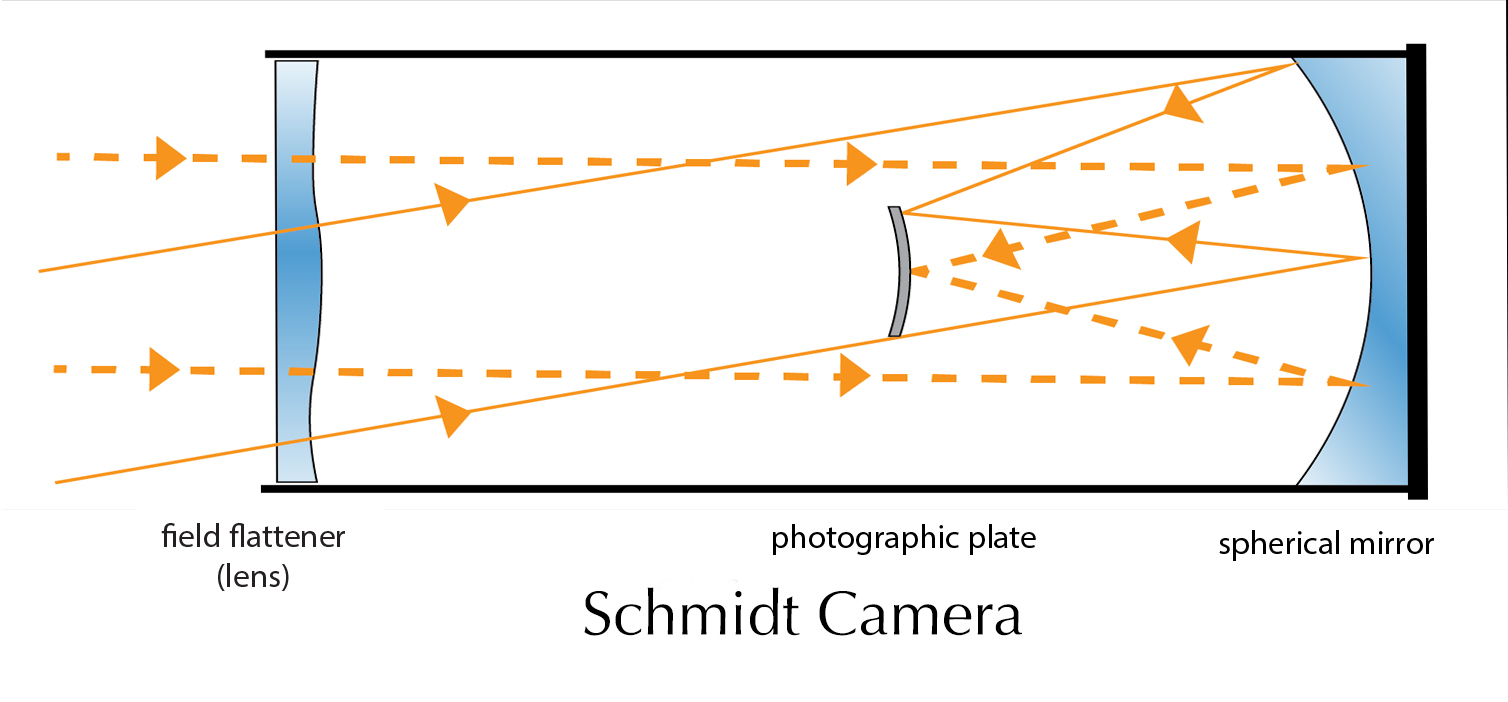
\includegraphics[width=0.7\linewidth]{Schmidt_Camera}
\end{figure}
		Широкоугольный телескоп, поле не менее $1^{\circ}$
		Корректирующая пластина Шмидта — это асферическая линза, которая корректирует сферическую аберрацию, возникающую из-за сферического первичного зеркала.\\
	\textbf{Оптическая схема менискового телескопа
		Максутова.}
\begin{figure}[h]
	\centering
	\includegraphics[width=0.7\linewidth]{"Снимок экрана от 2024-12-22 18-56-32"}
\end{figure}\\
Корректор с простыми сферическими поверхностями, если придать ему форму т.н.
ахроматического мениска, устраняет сферическую аберрацию зеркала.
\end{itemize}

Рефлектор – нет хроматизма.
Эллиптическое/параболическое зеркало – нет сферической абберации.

	\subsection{Конструкция телескопов и типы монтировок. Тонкие и сегментированные зеркала. Активная и адаптивная оптика.}
	
	Монтировка – фундаментальная часть телескопа, к которой навешивается труба. Она обеспечивает наведение трубы телескопа в нужное место небесной сферы и слежение за объектом, смещающимся из-за	суточного вращения Земли.
	
	\textbf{Параллактическая монтировка}, в которой вращение
	вокруг двух взаимно-перпендикулярных осей (полярной
	оси и оси склонения) позволяет осуществлять наведение.
	
	\textbf{Альт-азимутальная монтировка} -- одна из осей
	направлена по вертикали, вторая ось будет направлена
	по горизонтали. Для слежения за объектом требуется непрерывный пересчёт экваториальных
	координат в горизонтальные, вращения телескопа вокруг обеих осей.
	
	\textbf{Виды параллактических монтировок:}
	\begin{itemize}
		\item \textbf{Немецкая} -- С одной стороны оси склонения навешивается труба, с другой противовес,  чтобы обеспечить лёгкость вращения телескопа вокруг полярной оси. Процесс совмещения центра тяжести с точкой пересечения осей называется балансировкой телескопа. На низких широтах немецкая монтировка
		непригодна даже для малых телескопов.
		\item \textbf{Английская} -- Полярную ось устанавливают на двух колоннах (северной и южной), а ось склонения с	трубой и противовесом закрепляют на ее середине.
		\item \textbf{Американская (вилка)} -- Полярная ось	заканчивается вилкой, на концах	которой крепится
		ось склонения.
		\item \textbf{Комбинация английской монтировки и вилки} -- Ось склонения расположена внутри рамы, и
		на ней закреплена труба. Недостатком такой монтировки («качалки») является невозможность наведения	телескопа в область вблизи полюса мира.
	\end{itemize}
	
	\textbf{Зеркала}\\
	Просветление оптики -- уменьшение отражения света от поверхности линзы в результате нанесения на нее специальной пленки.\\
	\textbf{Сегментированные зеркала} -- изготовление больших монолитных зеркал является технически сложной задачей. Сегментированные зеркала позволяют обойти эти ограничения, так как каждый сегмент можно изготовить и полировать отдельно, а затем собрать их вместе. Большие монолитные зеркала могут деформироваться под воздействием температурных изменений, что снижает качество изображения. Сегментированные зеркала менее подвержены таким деформациям, так как каждый сегмент может быть откалиброван и подстроен независимо. егментированные зеркала могут быть использованы в системах адаптивной оптики, где каждый сегмент может быть динамически настроен для компенсации атмосферных искажений и других факторов, что позволяет улучшить качество изображения. Изготовление и полировка больших монолитных зеркал требует значительных затрат. Сегментированные зеркала могут быть более экономичными в производстве, так как каждый сегмент можно изготовить с использованием стандартных технологий и материалов.
	
	
	\textbf{Современные зеркала} -- Зависимость от температуры	коэффициентом расширения $20-120^{\circ}C=(28,39)\cdot10-7'/$град. веса.	Конструкция -- жесткая.	Механическая система
	разгрузки. \\
	\textbf{Тонкие зеркала} -- Поддержка тонкого зеркала, 150
	актюаторов (домкратов) расположены в 6-ти концентрических кругах. Зеркало должно быть тонким и лёгким!	Такое зеркало быстро принимает температуры окружающей среды. \newpage
		\textbf{Активная оптика} -- это автоматическая система для поддержания идеальной формы и правильного расположения оптических элементов телескопа-рефлектора,	прежде всего его главного и вторичного
		зеркал.\\
		\textbf{Адаптивная оптика} -- системы, способные в реальном времени компенсировать атмосферное размытие изображений. Метод предложил Хэролд Бэбкок 1953г.
		
		
\begin{figure}[h]
	\centering
	\includegraphics[width=0.5\linewidth]{"Снимок экрана от 2024-12-23 15-06-13"}
\end{figure}
	
	\textbf{Деформируемое зеркало} -- должно работать с высоким временным и пространственным разрешением, чтобы исправлять достаточно	малые участки волнового фронта! Размеры зеркала: 10 – 50 см. Делитель -- дихроичный фильтр, научная аппаратура и анализатор волнового фронта работают в разных диапазонах длин волн. Цикл измерений и коррекции действует очень быстро на аппаратуру и	поступает почти плоский волновой фронт. Восстанавливается исходная форма волнового фронта от объекта, несущая информацию о его структуре.
	
	\subsection{Солнечные телескопы. Целостат, внезатменный коронограф и космические солнечные телескопы.}
	
	\textbf{Целостатом} называется специальная установка с плоским вращающимся зеркалом, которое отражает пучок световых лучей звёзд или Солнца в заданном неизменном направлении, несмотря на видимое суточное перемещение светила.
	
\begin{figure}[h]
	\centering
	\includegraphics[width=0.9\linewidth]{"Снимок экрана от 2024-12-23 15-14-09"}
\end{figure}
	\newpage
	Универсальный автоматизированный солнечный телескоп с комплексом магнитографов и спектрофотометров.\\
	\textbf{Результаты наблюдений:}
	\begin{itemize}
	\item	Впервые была получена детальная картина всплытия магнитного поля активной области из
	нижних слоёв Солнца на поверхность, обнаружены новые закономерности структуры и
	динамики магнитного поля на разных стадиях эволюции активной области.
	\item Показано, что магнитный поток активной области не полностью диссипирует в процессе ее
	эволюции или покидает Солнце, а часть его погружается обратно в нижние слои Солнца.
	\item Обнаружены особые свойства конвективных движений в активной области - кольцевые
	конвективные структуры вокруг пятна, взаимодействие которых с магнитным полем определяет
	стабильность солнечных пятен, их эволюцию и время жизни.
	\end{itemize}
	\newpage
	
\begin{figure}[h]
	\centering
	\includegraphics[width=0.3\linewidth]{"Снимок экрана от 2024-12-23 15-21-34"}
\end{figure}
	
	\textbf{Внезатменный коронограф} состоит из главного объектива О, строящего изображение
	Солнца на металлическом диске Д, который не пропускает дальше свет
	фотосферы и создаёт таким образом искусственное затмение.
	Для устранения рассеянного света, появляющегося вследствие дифракции от края
	главного объектива, за металлическим экраном ставится линза О', которая строит
	изображение главного объектива на диафрагме В с отверстием достаточно малым,
	чтобы не пропустить изображение краёв главного объектива.
	Следующий объектив О'' строит окончательное изображение короны или
	протуберанцев на щели спектрографа или на фотоплёнке П. В последнем случае
	свет проходит через монохроматический
	интерференционно-поляризационный светофильтр Ф для устранения всех лучей,
	кроме спектральной линии, излучаемой короной или протуберанцем.
	Применение при наблюдениях специальных фильтров с уменьшающейся от центра к краям
	плотностью позволяет на одних и тех же фотографиях получать изображения яркой внутренней
	и более слабой внешней короны. Внезатменные К. обеспечивают наилучшие результаты при
	установке их в горах, где атмосферный рассеянный свет значительно меньше.
	В СССР первые наблюдения короны вне затмения были осуществлены на
	Кисловодской горной астрономической станции в 1950 на К. с диаметром объектива
	20 см. На этой станции, а также на обсерваториях вблизи Иркутска, в Абастумани и
	Алма-Ате находятся крупнейшие в мире К. с диаметром объектива 53 см.
	
\begin{figure}[h]
	\centering
	\includegraphics[width=0.6\linewidth]{"Снимок экрана от 2024-12-23 15-24-04"}
\end{figure}
	\textbf{Космические солнечные телескопы} -- телескопы, расположенные на орбите Земли или в других точках космического пространства, которые позволяют наблюдать Солнце без влияния земной атмосферы. Например,
	SOHO (Solar and Heliospheric Observatory): Запущенный в 1995 году, SOHO предоставляет данные о солнечной активности, короне и солнечном ветре.\\
	\textbf{Преимущества космических солнечных телескопов:}
	\begin{itemize}
	\item Отсутствие атмосферных искажений: Позволяет получать более четкие и детализированные изображения.
	\item Постоянное наблюдение: Возможность непрерывного мониторинга солнечной активности.
	\item Широкий спектральный диапазон: Возможность наблюдений в ультрафиолетовом, рентгеновском и других диапазонах, которые недоступны с Земли.
	\end{itemize}
	\subsection{Особенности ИК-телескопов. Телескопы для далекого ультрафиолета и рентгеновского излучения, космические ИК/УФ/X телескопы.}
	
	\textbf{ИНФРАКРАСНАЯ АСТРОНОМИЯ} - область наблюдательной
	астрофизики, объединяющая методы и результаты исследований
	излучения астр, объектов в ИК-диапазоне (0,7 мкм -- 1 мм). Иногда
	как часть выделяют субмиллиметровую астрономию (0,1 -- 1 мм).
	Первым шагом в истории И. а. было открытие ИК-излучения
	Солнца (У. Гершель, 1800).
	
	Спектр пропускания атмосферы в
	ближней и средней инфракрасной
	области (1,2 -- 40 мкм) на уровне моря
	(нижняя кривая на графиках) и на
	высоте 4000 м (верхняя кривая);
	в субмиллиметровом диапазоне (300 --
	500 мкм) излучение до поверхности
	Земли не доходит.
	\text{ИК -- излучение}
	\begin{itemize}
		\item Основной механизм генерации галактического ИК-излучения - тепловой;
		\item Главная излучающая субстанция - межзвёздная или околозвёздная пыль;
		\item Линейчатое излучение газа, обусловленное тонкой структурой уровней энергии атомов
		CI на волне $\lambda =157$ мкм, OI (63 мкм), OIII (88 мкм), Nell (12,8 мкм и др. и переходами между
		вращательно-колебательными и чисто вращательными уровнями энергии молекул (СО, $NH_3$,
		ОН, SiO, $Н_2$ и др.).
	\end{itemize}
	
	IRTF -- 3м телескоп, первый телескоп для наблюдений в близком инфракрасном свете.\\
	\textbf{Меры уменьшения фонового сигнала и корректного его
		учета:}
	\begin{itemize}
		\item Размер вторичного зеркала чуть меньше, чем требуется для получения невиньетированного
		изображения на оси;
		\item Для отражающих покрытий используется серебро или золото,
		имеющие меньшую по сравнению с алюминием излучающую способность;
	\item	Центральное отверстие в главном зеркале как раз достаточно для пропускания осевого пучка
		кассегреновского фокуса;
	\item	Фон неба отсекается коническим зеркалом, установленным в центре вторичного зеркала и
		закрывающим изображение отверстия в главном зеркале;
	\item	Вводятся охлаждаемые отсекатели и диафрагмы, которые экранируют все не отражающие
		поверхности в пучке света, собираемого телескопом;
	\item	Используется модулирующее вторичное зеркало с растяжками минимального сечения.
		Приборы для измерения инфракрасных лучей помещают в вакуум и охлаждают жидким гелием.
	\end{itemize}
	
	Спитцер (Spitzer) Выведен на орбиту в августе 2003 года.
	Оснащен 85-сантиметровым бериллиевым зеркалом, обеспечивающим
	разрешение до 1“. Охлаждение аппаратуры производится жидким гелием.
	Обсерватория Спитцер уникальна движется по гелиоцентрической орбите. Это
	было сделано для того, чтобы аппаратура остывала вдали от нашей планеты и
	была способна более точно улавливать сигналы, избегая помех.\\
	Используется для изучения самых далеких
	галактик.
	С помощью Спитцера было открыто
	2 внесолнечные планеты,
	несколько сверхмассивных черных дыр,
	а так же гигантские пылевые облака
	вокруг некоторых звезд.\\
	В 1983 году на околоземную орбиту был выведен
	знаменитый телескоп IRAS. Он проработал на орбите
	больше года, и основным его назначением было
	исследование излучения центральной области Млечного
	Пути.
	     
	     
	\textbf{Телескопы для далекого ультрафиолета (УФ)}\\
	\textbf{Особенности:}
	\begin{itemize}
	\item Детекторы: УФ-телескопы используют детекторы, чувствительные к ультрафиолетовому излучению. Эти детекторы часто изготавливаются из материалов, таких как фосфор или микроканальные пластины.
	\item Атмосферные окна: Земная атмосфера сильно поглощает ультрафиолетовое излучение, поэтому УФ-телескопы обычно размещаются в космосе.
	\item Оптика: УФ-телескопы используют специальные оптические системы, такие как зеркала с алюминиевым покрытием, которые эффективно отражают ультрафиолетовое излучение.\\
	
	Примеры космических УФ-телескопов:\\
	
	Hubble Space Telescope (HST): Хотя HST работает в нескольких диапазонах, включая видимый свет, он также оснащен УФ-детекторами.\\
	GALEX (Galaxy Evolution Explorer): Запущенный в 2003 году, GALEX изучал ультрафиолетовое излучение от галактик и звезд.
	\end{itemize}\newpage
	\textbf{Рентгеновские (X) телескопы}\\
	\textbf{Особенности:}
	\begin{itemize}
		\item Детекторы: Рентгеновские телескопы используют детекторы, чувствительные к рентгеновскому излучению, такие как газовые пропорциональные счетчики или полупроводниковые детекторы.
		\item Оптика: Рентгеновские фотоны имеют высокую энергию и требуют специальных оптических систем, таких как вольфрамовые зеркала, которые могут фокусировать рентгеновское излучение.
		\item Атмосферные окна: Земная атмосфера полностью поглощает рентгеновское излучение, поэтому рентгеновские телескопы должны быть размещены в космосе.\\
		
		Примеры космических УФ-телескопов:\\
		
		Chandra X-ray Observatory: Запущенный в 1999 году, Chandra предоставляет высококачественные изображения рентгеновских источников, таких как черные дыры и нейтронные звезды.\\
		XMM-Newton: Запущенный в 1999 году, XMM-Newton изучает рентгеновское излучение от различных космических объектов, включая галактики и звездные кластеры.
	\end{itemize}
	
	\subsection{Оптические интерферометры. Интерферометр Фабри - Перо.}
	
	\textbf{Оптические интерферометры}\\
	\textbf{Основные принципы:}
	Оптические интерферометры используют принцип интерференции света для получения высокоразрешающих изображений и спектров. Основные компоненты включают:
	\begin{itemize}
	\item Два или более телескопов: Разнесенные на значительное расстояние для создания длинной базы.
	\item Комбинатор: Устройство, которое объединяет свет от разных телескопов для создания интерференционной картины.
	\item Детекторы: Чувствительные приборы для регистрации интерференционных полос.
	\end{itemize}
	\textbf{Преимущества:}
	\begin{itemize}
\item	Высокое угловое разрешение: Оптические интерферометры могут достигать углового разрешения, значительно превышающего возможности традиционных телескопов.
\item	Спектральное разрешение: Возможность получения высокоразрешающих спектров, что важно для изучения химического состава и физических условий в космических объектах.
	\end{itemize}
	\textbf{Примеры использования:}\\
	VLTI (Very Large Telescope Interferometer): Часть Европейской южной обсерватории (ESO), используется для наблюдения звезд, экзопланет и других компактных объектов.\\
	CHARA (Center for High Angular Resolution Astronomy): Интерферометр, расположенный на горе Вильсон в Калифорнии, используется для изучения звездных поверхностей и двойных звезд.\\
	
	\textbf{Интерферометр Фабри-Перо}\\
	\textbf{Основные принципы:}
	Интерферометр Фабри-Перо состоит из двух параллельных полупрозрачных зеркал, разделенных воздушным зазором. Основные компоненты включают:
	\begin{itemize}
	
\item	Два зеркала: Одно частично отражающее, другое полностью отражающее.
	\item Воздушный зазор: Расстояние между зеркалами, которое можно изменять для настройки интерферометра на определенную длину волны.\\ 
\end{itemize}
	\textbf{Преимущества:}
	\begin{itemize}
\item	Высокое спектральное разрешение: Позволяет разрешать очень близкие спектральные линии, что важно для спектроскопии.
\item	Простота конструкции: Относительно простая и компактная конструкция, что делает его удобным для использования в различных приложениях.
\begin{figure}[h]
	\centering
	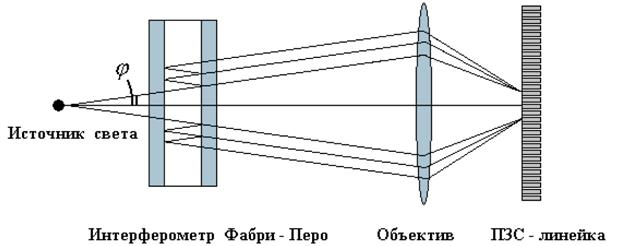
\includegraphics[width=0.7\linewidth]{image029}
\end{figure}


	
\end{itemize}
	\textbf{Примеры использования:}\\
	
	Спектроскопия: Используется для высокоразрешающей спектроскопии звезд, галактик и других космических объектов.\\
	Лазерная спектроскопия: Применяется в лабораторных условиях для изучения атомных и молекулярных спектров.\\
	
	Интерференционные фильтры -- интерферометры Фабри-Перо с
	интерференцией низкого порядка.
	
	Интерференция происходит в слое
	воздуха между двумя плоскими и
	параллельными друг другу
	поверхностями, покрытыми тонким
	полупрозрачным слоем
	серебра.
	
	
	\subsection{Фотометры, поляриметры, светофильтры.} 
	
	
	\textbf{Фотометрия} -- измерения света объекта, по полученным измерениям исследовать
	характеристики объекта.
	
	\textbf{Звёздная фотометрия} -- на основе многоцветной фотометрии звёзд восстановить
	распределение энергии в их спектрах, получить данные о температуре, светимости и
	химическом составе атмосферы звезды; звёздную величину в любой заданной полосе
	реакции приёмника. Изучение многочисленных и разнообразных эффектов переменности
	звёзд.
	
 	\textbf{Поверхностная фотометрия} -- один из наиболее распространённых и информативных
	методов исследования галактик. Фотометрический анализ позволяет получить
	информацию о распределении массы в галактиках, об их глобальной структуре и
	геометрических параметрах. Используя многоцветную фотометрию можно сделать
	заключение о звёздном населении галактик, об их пространственной ориентации, о наличии
	и характеристиках пылевой составляющей и т.д. её целью является измерение
	распределения яркости по поверхности протяжённого объекта.
	
	\textbf{Светофильтры} -- оптические приспособления, пропускающих свет
	определённых длин волн.
	
	\textbf{Использование светофильтров:}
	\begin{itemize}
		\item Оценка энергии, излучаемой источником в тех или иных областях
		спектра;
		 \item Выделение отдельных линий излучения газа ( выделяя излучение в
		линии $H_{\alpha}$, можно наблюдать солнечные протуберанцы вне затмений);
		\item  Устранение помех, вызванных свечением ночного неба;
		
		\textbf{Типы фильтров:}
		\begin{itemize}
		 \item Абсорбционные (поглощающие/пропускающие)
		\item Интерферометрические.
	\end{itemize}
\end{itemize}


\textbf{Стеклянные светофильтры} -- обычно представляют собой плоскопараллельные пластинки (или
системы пластинок).
\begin{itemize}
\item Пропускают излучение в широком диапазоне порядка 1000 А.
\item Материал – соли никеля или оксида кобальта растворённые в

\item стекле;
\item желатине;
\item коллоидном растворе (медный купорос – гасят пропускание в ИК).
	\end{itemize}
Все стеклянные С. непрозрачны для далёкого УФ- и ИК-излучения.

\textbf{Нейтральные фильтры для наблюдений Солнца,
Луны.} -- служат для ослабления яркого солнечного
света, обычно в несколько десятков тысяч раз.
Конструктивно фильтр обычно представляет
собой стеклянную пластинку или
синтетическую пленку, покрытую тонким слоем
металла.

\textbf{Дихроичные фильтры} -- пропускают в одном диапазоне и отражают в другом.

\textbf{Абсорбционные фильтры}, характеризуются резким изменением
коэффициента поглощения в определённом спектральном диапазоне.

Односторонние фильтры гасят
коротковолновое и пропускают
длинноволновое излучение, начиная с
некоторой длины волны (в зависимости
от марки стекла).


Двусторонние фильтры могут
быть центрированы на разные
длины волн и иметь разную
ширину полосы пропускания (но
всегда порядка нескольких сот
ангстрем).


\textbf{Электрофотометры}.
\begin{itemize}
\item Объектив строит в фокальной плоскости, где помещена диафрагма,
изображение источника.
\item Диафрагма вырезает световой поток которой нужно измерить.
Набор нескольких диафрагм различного диаметра (от 1-2" до 1'),
которые применяются в зависимости от поставленной задачи и
объекта наблюдения.
\item Перед диафрагмой для наводки на объект или нужное место диска
планеты устанавливается подсмотр, состоящий из откидного
зеркала и слабого широкоугольного окуляра с крестом нитей,
согласованным с центром диафрагмы.
\item Для контроля положения источника в фокальной диафрагме
применяется другой подсмотр, состоящий из выдвижной призмы П
и микроскопа О1О2.
\item Призма
\item Рамка со светофильтрами.
\item  Линза Фабри обеспечивает правильное освещение фотокатода
ФЭУ светом от исследуемого объекта.
\end{itemize}

\textbf{Поляриметры.}
\begin{itemize}
\item  Поляризация в космических условиях возникает повсеместно: при рассеянии, при нетепловом
механизме излучения, при распространении излучения в плазме и т.д. В тех случаях когда она
обнаружима, измерение величины, изменения ее во времени и с длиной волны, позволяет сделать
важные выводы о физических условиях в месте формирования излучения. \newpage


\textbf{ Метод измерения поляризации излучения небесных тел:}
\item  Поляриметры – приборы, обнаруживающие поляризованное излучение и некоторые его
характеристики. В основном из наблюдений можно получить степень линейной поляризации и
направление.
\item  Цель – получить параметры Стокса.
\item  Поляроиды
\item  призма Воластона, пластина Саварра.
\end{itemize}
	\subsection{Спектрографы. Оптическая схема, призмы и дифракционные решётки. Мультизрачковый и мультиобъектный спектрографы.}
	
	\textbf{Спектроскопия} – разложение света по длинам волн на его
	монохроматические составляющие.
	
	\begin{itemize}
	
\item Измерение красного смещения;
	\item Определение типа объекта;
\item Измерение лучевых скоростей: кинематика звёзд и газа (туманности и
	галактики) ;
\item Химический состав и возраст звёздного населения;
\item Химический состав газовой составляющей, физические условия ($T_e$, $n_e$) в областях формирования эмиссионных линий.
\end{itemize}


\textbf{Типы спектроскопии:}
	\begin{itemize}
\item Щелевая;
	\begin{itemize}
\item Дифракционные решётки;
\item Голографические решётки;
\item Призма;
\end{itemize}
\item Бесщелевая;
\item Панорамная;
	\begin{itemize}
\item Многощелевая; 
\item мультиобъектная;
\item Мультизрачкавая;
\item Интерферометер Фабри - Перо.
\end{itemize}
\end{itemize}
\newpage
\begin{figure}[h]
	\centering
	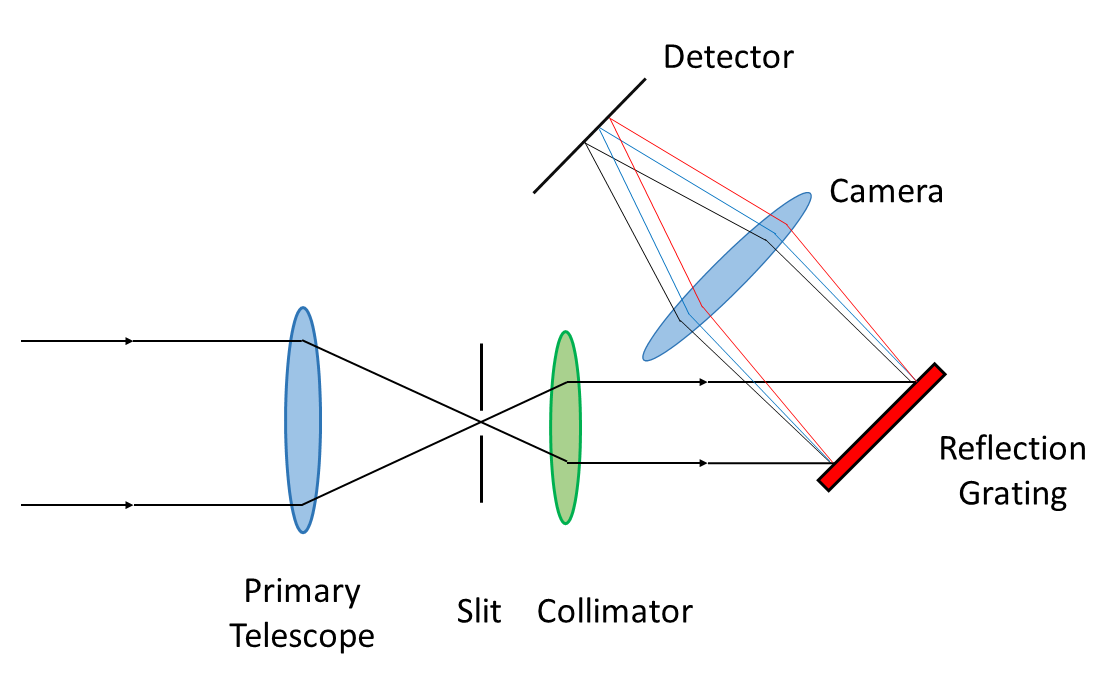
\includegraphics[width=0.7\linewidth]{Схема_спектрографа_с_дифракционной_решеткой}
\end{figure}
Спектрограф строит серию монохроматических изображений входной
щели, поэтому для нас важно только то, что решетка разводит лучи с
разными длинами волн, т.е. обладает дисперсией.

Для отсутствия световых потерь и полного использования диаметра
объектива спектрографа его относительное отверстие должно быть равно
относительному отверстию телескопа.

\textbf{Требования к коллиматору и камере.}
\begin{itemize}
\item Коллиматор должен создавать параллельный пучок для всех длин волн, у
него не должно быть хроматической аберрации.
Наряду со сложными линзовыми системами используются зеркальные
коллиматоры (полностью свободные от хроматической аберрации) типа
обратного Кассегрена.
\item Для объектива камеры хроматизм несущественен он легко убирается
наклоном приёмника. Основные требования к объективу камеры –
большое безаберрационное поле и хорошая светосила.
\end{itemize}



\textbf{Мультизрачковые спектрографы}

Основные принципы:

	Мультизрачковые спектрографы позволяют одновременно получать спектры нескольких объектов или нескольких точек одного объекта.
\begin{itemize}
\item Оптическая схема: Включает несколько входных щелей или волокон, которые направляют свет от разных объектов или точек в один спектрограф.
\item Преимущества: Повышенная эффективность наблюдений, возможность одновременного анализа нескольких объектов.
\end{itemize}
Примеры использования: Изучение звездных скоплений, галактик и других объектов, требующих одновременного анализа нескольких точек.

\textbf{Мультиобъектные спектрографы}

Основные принципы:

Мультиобъектные спектрографы позволяют одновременно получать спектры множества объектов в одном поле зрения.
\begin{itemize}
\item Оптическая схема: Включает маску с множеством щелей или волокон, которые направляют свет от разных объектов в спектрограф.
\item Преимущества: Высокая эффективность наблюдений, возможность одновременного анализа большого числа объектов.
\end{itemize}
Примеры использования: Изучение больших звездных скоплений, галактик и других объектов, требующих одновременного анализа множества объектов.



\textbf{Призмы и дифракционные решётки}
\textbf{Призмы:}

Принцип работы: Призмы используют преломление света для разложения его на спектральные компоненты. Свет проходит через призму и изменяет направление в зависимости от длины волны.

Преимущества: Простота конструкции и высокая пропускная способность.

Недостатки: Ограниченное спектральное разрешение и нелинейная дисперсия.

\textbf{Дифракционные решётки:}

Принцип работы: Дифракционные решетки используют интерференцию света для разложения его на спектральные компоненты. Свет проходит через решетку и дифрагирует на разные углы в зависимости от длины волны.

Преимущества: Высокое спектральное разрешение и линейная дисперсия.

Недостатки: Меньшая пропускная способность по сравнению с призмами.
	\section{Блок. Приёмники излучения.}
\subsection{Основные типы и основные характеристики и ограничения приемников излучения, типы шумов.}
\textbf{Поглощение излучения}
\begin{itemize}
	\item Нагрев;
	\item Фотоэлектрические явления;
	\item Фотохимические явления;
	\item Вторичное излучение;
		\begin{itemize}
			\item Тепловое излучение;
			\item Люминесценция;
			\item Индуцированное излучение.
	\end{itemize}
	
\end{itemize}
Некогерентные регистрируют только амплитуду излучения,
информация о фазе теряется.\newpage
\textbf{Типы детекторов:}
\begin{itemize}
	\item \textbf{Фотонные приемники} -- отклик прибора на фотон:
		\begin{itemize}
			\item Физические процессы на микроскопических уровнях;
			\item Поглощённый фотон взаимодействует напрямую с электронами приёмника
			производит один/несколько заряженных частиц в приёмнике:
			\begin{itemize}
				\item Изменяют характеристики электрического тока;
				\item Сразу проходят на усилители;
				\item Приводят к химическим реакциям.
			\end{itemize}	
			Применяются от рентгеновского диапазона до инфракрасного. Примеры: глаз, фотографическая эмульсия, фотоумножители, фотодиоды, счетчики фотонов, CCD.
			\end{itemize}	
	\item \textbf{Тепловые приёмники} -- в большинстве случаев
	падающее излучение изменяет их электрические
	свойства, проводимость.
			\begin{itemize}
			\item Физические процессы проходят на макроскопическом уровне,
			регистрируют излучение по увеличению температуры. Менее
			чувствительные и медленнее.	
			
		Применяются в инфракрасном и субмиллиметровом
		диапазоне и рентгене. Примеры: болометры, термопары.
		\end{itemize}	
	\item \textbf{Когерентные} -- регистрируют не только силу электрического поля
	сигнала, но и информацию о фазе. Регистрация сигнала происходит на
	основе интерференции приходящего излучения с когерентным
	осциллятором.
	применяют в радио и субмиллиметровом
	диапазоне.
	
	
	\textbf{Характеристики приёмников}
	\begin{itemize}
		\item Спектральная чувствительность -- диапазон длин волн в котором фотон может быть зарегистрирован на значимом уровне;
		\item Спектральная полоса пропускания -- диапазон длин волн в котором одновременно регистрируются фотоны;
		\item  Линейность -- зависимость выходного сигнала на падающее излучение;
		\item	Динамический диапазон -- диапазон изменения сигнала, который регистрируется без потери информации;
		\item Квантовая эффективность -- отношение принятого количества фотонов к количеству преобразованных в сигнал;
		\item Шум -- неопределённость в выходном сигнале;
		\item Временной отклик -- минимальный временной интервал, в котором приёмник регистрирует
		приходящее излучение;
		\item Панорамные свойства -- количество элементов, строящих изображение на приёмнике;
		\item Частотно -- контрастная характеристика -- отражает
		возможность оптической
		системы передать контрастное изображение
		снимаемого объекта.
	\end{itemize}
\end{itemize}

\textbf{Шумы}
\begin{itemize}
	\item По месту возникновения:
		\begin{itemize}
		\item Фотонный или радиационный шум сигнала;
			Среднеквадратичная ошибка одного измерения (Корень из n)
		\item Внесённый земной атмосферой (флюктуации яркости ночного
		неба);
		\item Шумы приёмника (фоновый характер, изменения темнового
		тока);
		\item Шумы, вносимые измерительной/усилительной техникой.
		\end{itemize}
	\item По внутренней природе шумы разделяют:
	\begin{itemize}
		\item Дробовые; 
			Если процесс имеет дискретную природу, то появляется дробовой шум:
			\begin{itemize}
			\item беспорядочные флуктуации напряжений и токов относительно их среднего значения.
			Возникают в цепях электронных устройств и обусловлены дискретностью самих
			носителей электрического заряда, то есть ионов и электронов. Поэтому перемещение
			каждого носителя заряда в общей цепи сопровождается всплеском тока;
			\item дискретное количество падающих фотонов (фотонный шум).
			\end{itemize}
		\item Тепловые;
		Тепловые шумы вызываются хаотическим тепловым движением свободных электронов
		проводящего материала приёмника. В результате такого движения, число электронов,
		перемещающихся в одном направлении, не равно числу электронов, движущихся в
		противоположном направлении. В результате, возникающий в нагрузке ток или напряжение
		носит случайный характер. 
		
		Тепловой шум присущ только проводникам и его среднеквадратичное отклонение
		определяется формулой Найквиста:
		 $$\sigma_U=\sqrt{4kTR_T\Delta f}$$
		 T -- температура чувствительного слоя приемника в Кельвинах; $R_T$ -- сопротивление при данной температуре; $\Delta f$ -- полоса частот, в которой измеряется среднеквадратичное отклонение.
		\item Низкочастотные; Этот шум проявляется в детекторах излучения на низких частотах. Обычно появление этих
		шумов связывают с наличием потенциальных барьеров на контактах, в объёме или на
		поверхности полупроводника. Для монокристаллических полупроводников с омическими
		контактами эти шумы в основном связаны с процессами на поверхности. 
		В фотоэмиссионных приборах эти шумы наблюдаются в виде шумов мерцания, связанных с
		термоионной эмиссией, с эмиссией в сильном электрическом поле или утечками от анода к
		катоду.
		\item Шумы, вызванные паразитными явлениями в приёмниках.
	\end{itemize}
\end{itemize}

\begin{itemize}
	\item У термоэлементов преобладают тепловые шумы;
		\item у полупроводниковых болометров – тепловые и токовые;
			\item У фоторезисторов – токовые и радиационные;
				\item При наличии нескольких шумовых механизмов их общее
				среднеквадратичное значение может быть вычислено
				суммированием их дисперсий;
				
\end{itemize}

\textbf{Фотографическая пластинка} представляет собой полированное стекло,
покрытое желатиновым эмульсионным слоем, содержащим
светочувствительные кристаллы галоидного серебра (обычно AgBr).
При освещении эмульсии электроны отрываются от ионов Br и закрепляются
на неоднородностях кристаллической решетки, туда притягиваются ионы
серебра, образуются атомы серебра, на которых закрепляются электроны,
притягивающие ионы серебра, превращающиеся в атомы и т.д.

Нерегулярность распределения светочувствительных зерен в эмульсии приводит:
\begin{itemize}
\item зернистости изображения;
\item появление шумов при определении плотности.
\end{itemize}


Малая чувствительность:
\begin{itemize}
	\item Число фотонов, поглощенных активным веществом эмульсии, составляет около 0.1 от числа
	падающих фотонов (0.4 отражается от эмульсионного слоя или проходит его, не встречаясь с
	активным веществом; 0.5 рассеивается и поглощается желатином);
	\item для того, чтобы зерно могло проявиться, на него должно упасть не меньше 10 фотонов;
	\item В результате эффективность -- 0.01, Квантовый выход в максимуме – около 1\%
\end{itemize}
Малая чувствительность отчасти компенсируется тем, что фотографический эффект
накапливается при увеличении выдержки.
\subsection{Приемники излучения, работающие на внешнем фотоэффекте.}
Внешний фотоэффект, или фотоэлектронная эмиссия – это испускание электронов с поверхности
фоточувствительного слоя в вакуум или другое вещество под действием падающего потока излучения.
$$E_f > A + m\frac{v^2}{2}$$
A -- работа выхода электрона из вещества. $h\nu_{min}\ge A$
Минимальная частота квантов, способных
произвести фотоэффект определяет красную границу чувствительности приемника.
\begin{figure}[h]
	\centering
	\includegraphics[width=0.5\linewidth]{"Снимок экрана от 2024-12-23 18-41-39"}
\end{figure}
Диэлектрики не применяются!(ничтожно малая проводимость)

Самый высокий энергетический уровень потенциальной
ямы металла, занятый электронами при Т = 0, называется
уровнем Ферми.
У металлов высокая отражательная способность,
большие потери энергии при прохождении через
кристаллическую решетку столкновения со
свободными электронами – малая эффективность
в оптике.
Используются в УФ приемниках.

Наиболее эффективные фотокатоды
в оптике -- полупроводники.
\begin{itemize}
	\item эффективно поглощают фотоны;
	\item мало свободных электронов;
	\item поверхностный потенциал можно
	уменьшить.
\end{itemize}

\begin{figure}[h]
	\centering
	\includegraphics[width=0.5\linewidth]{"Снимок экрана от 2024-12-23 18-45-34"}
\end{figure}
Значения работы выхода для донорного а), собственного б) и акцепторного в) полупроводников.

Применение акцепторной примеси (p)
повышает квантовый выход.
Плёнка $Сs_2О$ уменьшает
Av и сдвигает длинноволновую границу.
Фотокатоды с отрицательной энергией
электронного сродства ($\chi$ < 0)

\textbf{Фотоэлектрические приборы}
\begin{itemize}
	\item  одноканальные – измеряется интегральный поток;
	\item  многоканальные.
\end{itemize}

Простейший одноканальный приемник -- \textbf{вакуумный фотоэлемент}.
В фотоэлектронных умножителях (ФЭУ) происходит усиление сигнала за счет
вторичной электронной эмиссии.
Явление вторичной электронной эмиссии состоит в том, что при бомбардировке
твердого тела
электронами, обладающими достаточной энергией, происходит испускание вторичных
электронов и на каждый первичный электрон приходится больше двух вторичных.
Начиная с 30-40-х гг. прошлого столетия и по настоящее время, ФЭУ широко
используются при наблюдениях в видимом и УФ диапазонах.
\begin{figure}[h]
	\centering
	\includegraphics[width=0.7\linewidth]{"Снимок экрана от 2024-12-23 18-51-48"}
\end{figure}\\
Назначение динодных систем – собрать все электроны с предыдущего
\begin{figure}[h]
	\centering
	\includegraphics[width=0.4\linewidth]{"Снимок экрана от 2024-12-23 18-53-37"}
\end{figure}

Искривленные каналы, чтобы уменьшить
бомбардировку катода ионами.
\begin{figure}[h]
	\centering
	\includegraphics[width=0.4\linewidth]{"Снимок экрана от 2024-12-23 18-53-44"}
\end{figure}\newpage
Усиление электронного потока при использовании непрерывного (канального)
динода: 1-фотокатод; 2-канал; 3-анод.


\textbf{Спектральная
чувствительность
ФЭУ} определяется
спектральной
чувствительность
ю фотокатода.
\begin{figure}[h]
	\centering
	\includegraphics[width=0.7\linewidth]{"Снимок экрана от 2024-12-23 18-55-53"}
\end{figure}\\
Спектральные характеристики фотокатодов: I - кислородно-цезеевый,
II-IV -сурьмяно-цезиевые разного типа, V – висмуто-цезиевый


\textbf{Основные параметры ФЭУ.}
\begin{itemize}
	\item Шумы -- ложные импульсы от космических лучей и распада радоиактивных
	изотопов в материале окошка.
	\item Термоэлектронная эмиссия с фотокатода и первого динода --
	охлаждение.
	
	ФЭУ моно использовать в двух режимах:
	\begin{itemize}
	\item Режим постоянного тока;
	\item Метод счета фотонов.
	\end{itemize}
\end{itemize}


\textbf{Многоканальные приемники}
В многоканальных приемниках на внешнем фотоэффекте строится электронное
изображение.
По способу его регистрации приемники делятся на следующие группы:
\begin{itemize}
	\item \textbf{Электронная камера} -- приемник, у которого электронное изображение строится на
	электронографической эмульсии;
	\item \textbf{Электронно-оптический преобразователь (усилитель яркости)} -- однокамерный или
	многокамерный прибор, строящий электронное изображение на флюоресцирующем
	экране;
	\item \textbf{Суперортикон - телевизионная трубка}, у которой электронное изображение
	строится на мишени, где в результате вторичной электронной эмиссии образуется
	потенциальный рельеф, который считывается электронным лучом.
\end{itemize}

\textbf{Приборы, строящие электронное
изображения.}
\begin{itemize}
	\item Катод;
	\item Фокусирующая система (магнитная или электростатическая);
	\item Ускоряющее напряжение;
	\item Анод.
\end{itemize}

\subsection{Одноканальные приемники на внутреннем фотоэффекте. Тепловые приемники.}
\textbf{Внутренний фотоэффект} -- происходит только изменение
энергетического состояния электронов, приводящее к
изменению концентрации носителей тока, их подвижности
или к перераспределению внутри объёма полупроводника.

Можно обнаружить:
\begin{itemize}
	\item  по возникновению разности потенциалов между участками освещённого
	полупроводника (Фото э.д.с. – фотогальванический эффект.)
	\item по изменению проводимости материала при его освещении (Фотопроводимость)
\end{itemize}

Полупроводники с собственной проводимостью: носители двух типов (электроны и дырки); движение электронов проводимости и дырок в отсутствие электрического поля является хаотическим.

Примером собственных полупроводников химически чистые Ge, Si, а также
многие химические соединения: InSb, GaAs, CdS и др.\\
\begin{figure}[h]
	\centering
	\includegraphics[width=0.3\linewidth]{"Снимок экрана от 2024-12-23 19-12-32"}
\end{figure}\\
Уровень Ферми в твёрдом теле при тепловом равновесии
всюду одинаков.
Объёмная концентрация электронов в зоне проводимости -- n,
дырок в валентной зоне -- p:
$$n = AT^{\frac{3}{2}}e^{\frac{E_F-E_2}{kT}}$$
$$p = BT^{\frac{3}{2}}e^{\frac{E_1-E_F}{kT}}$$
$$np = ABT^{3}e^{\frac{-E_G}{kT}}$$
$E_G$ -- слабо зависит от температуры. Определяет область применения полупроводника.

Если на кристалл наложить
электрическое поле, то электроны
начнут двигаться против поля, дырки
-- по полю, что приведёт к
возникновению собственной
проводимости германия,
обусловленной как электронами, так
и дырками.

Собственные полупроводники –
элементы IV группы (Si, Ge).

\textbf{Примесная проводимость} обусловлена
\begin{itemize}
\item примесями (атомы посторонних элементов);
\item дефектами типа избыточных атомов (по сравнению со
стехиометрическим составом);
\item тепловыми (пустые узлы или атомы в междоузлиях) и механическими
(трещины, дислокации и т.д.) дефектами;
\end{itemize}
Наличие в полупроводнике примеси существенно изменяет его проводимость.
Например, при введении в кремний примерно 0,001 ат. \% бора его
проводимость увеличивается примерно в $10^6$
раз.

Носители одного типа.

Введение примеси искажает поле решётки, что
приводит к возникновению в запрещённой зоне
энергетического уровня D валентных электронов
мышьяка, называемого примесным уровнем.

\begin{figure}[h]
	\centering
	\includegraphics[width=0.2\linewidth]{"Снимок экрана от 2024-12-23 19-20-02"}
\end{figure}


В случае германия с примесью мышьяка этот уровень
располагается от дна зоны проводимости на
расстоянии $\Delta E_D = 0.013$ эВ.

Так как  $\Delta E_D < kT$ , то уже при обычных температурах
энергия теплового движения достаточна для того,
чтобы перебросить электроны примесного уровня в
зону проводимости; образующиеся при этом
положительные заряды локализуются на неподвижных
атомах мышьяка и в проводимости не участвуют.

В полупроводниках с примесью, валентность которой на единицу
больше валентности основных атомов, носителями тока являются
электроны;возникает электронная примесная проводимость
(проводимость n-типа).
Полупроводники с такой проводимостью называются электронными
(или полупроводниками n-типа).
Примеси, являющиеся источником электронов, называются донорами,
а энергетические уровни этих примесей - донорными уровнями.\\
\textbf{Дырочная проводимость (проводимость р-типа)}\\
\begin{figure}
	\centering
	\includegraphics[width=0.2\linewidth]{"Снимок экрана от 2024-12-23 19-22-46"}
\end{figure}

Введение трехвалентной примеси в решетку
кремния приводит к возникновению в
запрещенной зоне примесного энергетического
уровня А, не занятого электронами. В случае
кремния с примесью бора этот уровень
располагается выше верхнего края валентной
зоны на расстоянии $\Delta E_A= 0.08$ эВ.

Близость этих уровней к валентной зоне приводит
к тому, что уже при сравнительно низких
температурах электроны из валентной зоны
переходят на примесные уровни и, связываясь с
атомами бора, теряют способность перемещаться
по решетке кремния, т.е. в проводимости не
участвуют. Носителями тока являются лишь
дырки, возникающие в валентной зоне.

В полупроводниках с примесью, валентность которой на
единицу меньше валентности основных атомов, носителями
тока являются дырки; возникает дырочная проводимость
(проводимость р-типа).

Полупроводники с такой проводимостью называются
дырочными (или полупроводниками р-типа).

Примеси, захватывающие электроны из валентной зоны
полупроводника, называются акцепторами, а энергетические
уровни этих примесей — акцепторными уровнями.


\textbf{Одноканальные приёмники}:
\begin{itemize}
	\item фотосопротивления (ФС);
	\item вентильные фотоэлементы;
	\item фотодиоды.
\end{itemize}
\textbf{Многоканальные}:
\begin{itemize}
	\item фотодиодные матрицы;
	\item приборы с переносом заряда (ПЗС);
\end{itemize}
В основном эти приёмники используются в ИК области.
Приёмники с зарядовой связью (ПЗС) работают \textbf{от рентгена до ИК диапазона}.

Полупроводниковое устройство,
содержащее один р-n -- переход или с
барьером Шоттки, называется
\textbf{полупроводниковым (кристаллическим)
диодом}.

Граница соприкосновения двух
полупроводников, один из которых имеет
электронную, а другой -- дырочную
проводимость, называется электронно-
дырочным переходом (или р-n-переходом).

р-n-переход нельзя осуществить просто механическим соединением двух
полупроводников.
Обычно области различной проводимости создают либо при выращивании кристаллов,
либо при соответствующей обработке кристаллов: дифференциального легирования
однородного кристалла полупроводника.

\textbf{Легирование} – введение контролируемого количества примесных атомов кристаллическую решётку.

В силу односторонней проводимости р-n-перехода при
его освещении в разомкнутом состоянии на электродах
появится э.д.с. (фотогальванический режим).

Если замкнуть электроды на последовательные
питание и нагрузку, изменится значение обратного тока
(фотовольтаический режим и его частный случай
лавинный режим).
Наибольшее распространение получили фотодиоды из германия (ширина
запрещенной зоны 0.67эв) и кремния (1.11эв).

Кремниевые фотодиоды изготавливаются с диффузионным p-n переходом.
Пластинка монокристаллического Si n-типа припаивается к металлическому
основанию, ее наружная поверхность покрывается слоем двуокиси кремния, в
котором вытравливается окно.
Диффузия акцепторной примеси р-типа в поверхностный слой кремния
осуществляется прогревом заготовки в атмосфере газа, содержащего соединения
бора.
В результате образуется слой р-типа, к которому припаивается электрод.\\


\textbf{Фотодиоды. P-I-N – переход} 
Positive – intrinsic – negative
PIN – диод.
Структура p-i-n представляет
собой собственный
полупроводник i с удельным
сопротивлением, в миллион и
более раз превышающим
удельное сопротивление у

сильно легированных n- и р-
слоев, ограничивающих его с

противоположных сторон.
Снаружи на эти слои наносят
контакты.
\begin{figure}[h]
	\centering
	\includegraphics[width=0.7\linewidth]{"Снимок экрана от 2024-12-23 19-34-25"}
\end{figure}\\
\textbf{Утолщение обеднённого слоя}.\\
Вероятность захвата фотона
увеличивается. (ближний ИК).
Уменьшается ёмкость –>
сокращается время реакции
более чувствительный приемник.

Фоторезистор – это полупроводниковый прибор,
проводимость которого изменяется в зависимости от
изменения падающего на него светового потока.
Фотосопротивления, используемые в астрономии,
работают при глубоком охлаждении.
Фоточувствительный слой монтируется в дно
дюаровского сосуда, который заполняется
углекислотой, жидкими азотом, гелием или другими
хладогентами, в зависимости от того, какая рабочая
температура необходима.

\textbf{БОЛОМЕТР} - устройство для измерения
потока энергии эл.-магн. излучения,
основанное на изменении физ.
параметров термочувствительного
элемента в результате его нагрева при
поглощении энергии измеряемого
излучения (тепловой приёмник
излучения).
В астрономии чаще всего используют для
регистрации ИК-излучения.

Применяются два типа: работающие при
комнатной температуре и при
охлаждении.

\subsection{ПЗС и ПЗС-матрицы.}
Приборы с зарядовой связью (ПЗС или CCD – Charge Coupled Device) –
это твердотельные матричные приёмники.
Преимущества:
\begin{itemize}
\item высокий квантовой выход;
\item широкий динамический диапазон;
\item низкий уровень шумов.
	В настоящее время широко используются в наблюдательной астрономии.
\end{itemize}


\textbf{МОП – конденсаторы}.
Подложка p – Si;Изолирующий слой $SiO_2$
(0.1 мкм); Металлический электрод
(затвор)

Металл – Окисел – Полупроводник

Инверсионный слой (слой с
обратной проводимостью)
вблизи границы раздела
толщиной $\approx$10 нм.

При $Т \approx 300$ К
термоэлектроны стекают в
переход.

При$Т \approx 10$0 К – инверсионный
слой образуется при появлении
фотоэлектронов.
\begin{figure}[h]
	\centering
	\includegraphics[width=0.3\linewidth]{"Снимок экрана от 2024-12-23 19-44-10"}
\end{figure}
Количество «жидкости в ведре»
соответствует величине заряда в
потенциальной яме. положение «поверхности жидкости»
показывает, на какую величину
уменьшился поверхностный
потенциал.

\begin{figure}[h]
	\centering
	\includegraphics[width=0.5\linewidth]{"Снимок экрана от 2024-12-23 19-45-06"}
\end{figure}
Поликристаллический кремний
\begin{itemize}
	\item обладает свойствами
	металлов;
	\item прозрачен, пропускание света;
	\item уменьшает опасность
	загрязнения.
\end{itemize}

ПЗС состоят из набора ячеек – МОП — конденсаторы.
Несколько МОП-конденсаторов на
одной подложке расположены так
близко, что обеднённые области
и потенциальные ямы перекрываются
тогда можно осуществить
управляемый перенос заряда.
\begin{figure}[h]
	\centering
	\includegraphics[width=0.4\linewidth]{"Снимок экрана от 2024-12-23 19-46-43"}
\end{figure}\\
\textbf{Трехфазный ПЗС приемник.}

Принцип работы трёхфазного ПЗС приёмника.
Цикл из трёх тактовых шагов повторяется, заряд перемещается по каналу
переноса до тех пор, пока не достигнет оконечного затвора.
В случае трёхфазного ПЗС каждая тройка затворов образует один
приёмный элемент.
Работает в обоих направлениях.
Основной недостаток трёхфазного прибора заключается в необходимости
трех последовательностей перекрывающихся тактовых импульсов.\newpage

\begin{figure}[h]
	\centering
	\includegraphics[width=0.5\linewidth]{"Снимок экрана от 2024-12-23 19-48-04"}
\end{figure}
\textbf{Двухфазный ПЗС приемник.}

Используются поликремниевые электроды,
часть из них погружена в окисел, и поэтому
потенциальные ямы глубже.
При подаче напряжения образуются
двухъярусные несимметричные потенциальные ямы, в которых будут накапливаться
заряды.
У
\begin{figure}[h]
	\centering
	\includegraphics[width=0.4\linewidth]{"Снимок экрана от 2024-12-23 19-48-42"}
\end{figure}
Величина накопительной ёмкости меньше;движение заряда возможно только в одном направлении.
Управление двухфазным ПЗС проще, и напряжения на фазах Ф1 и Ф2
могут быть просто противофазными и подаваться от одного генератора.


\textbf{Стоп -- диффузия} (стоп-каналы) -- узкие полоски с повышенной
концентрацией основной легирующей примеси. (локальное
увеличение проводимости между соседними каналами )
Поверхностный потенциал на границе раздела окисел --
кремний всегда близок к нулю, что препятствует растеканию
заряда.

\textbf{эффективность переноса и максимальная частота
переноса.}
частота переноса:

-- max ограничена подвижностью зарядовых пакетов между
ячейками,

-- min при охлаждении практически не ограничен.

Эффективность переноса – близка к 99.95, но
-- х 500 элементов – > сильное размытие изображения
-- ЭП-- 99.999!


Главным недостатком ПЗС с поверхностным каналом является наличие ловушек на
границе раздела $Si$ – $SiO_2$, что приводит к отличию эффективности переноса заряда
(ЭПЗ) от единицы.

Ловушки: наличие дефектов кристалла кремния. Часть заряда задерживается в
ловушках, это особенно сказывается при малых световых потоках, когда ловушки не
заполнены.

Один из способов борьбы – непрерывная слабая засветка, которая позволяет
поддерживать ловушки заполненными. Этот искусственный сдвиг называют
«жирным нулем». В астрономии роль «жирного нуля» играет фон неба.


\textbf{ПЗС с внутренним каналом.}
Между–кремнием и окислом
находится слой сильно
легированного кремния с другим
типом проводимости (n-типом).
Образуется p–n переход,
который смещают в обратном
направлении, прикладывая к n–
слою положительное
относительно подложки
напряжение.

\textbf{Преимущества:}
\begin{itemize}
	\item Количество ловушек в объёме кристалла гораздо меньше, чем на
	поверхности, поэтому значительно улучшается эффективность
	переноса, что особенно важно для малых зарядовых пакетов;
	\item Силовые линии электрического поля между соседними
	электродами почти параллельны направлению движения заряда;
	что ускоряет движение электронов.
	\item доступность работы с очень малыми сигналами расширяет
	динамический диапазон и увеличивает чувствительность ПЗС с
	внутренним каналом.
\end{itemize}

Главный недостаток ПЗС с внутренним каналом: 

уменьшение в 3-4 раза по сравнению с ПЗС с внешним каналом
накопительной ёмкости ячейки.

\textbf{Метод считывания зараяда.}
\begin{figure}[h]
	\centering
	\includegraphics[width=0.3\linewidth]{"Снимок экрана от 2024-12-23 20-00-48"}
\end{figure}

\begin{figure}[h]
	\centering
	\includegraphics[width=0.3\linewidth]{"Снимок экрана от 2024-12-23 20-03-43"}
\end{figure}
Не существует такого покрытия, которое одинаково
эффективно во всем спектральном диапазоне!

\textbf{Как повысить квантовый выход в УФ области:}
Использование поликремниевых электродов.
Нанесения отрицательного заряда, который создает
электрическое поле, отталкивающее электроны от
поверхности вглубь кристалла (тонкие ПЗС);
Нанесение на поверхность пленки с люминофором,
который поглощает коротковолновые фотоны и
переизлучает их в области около 500 нм.
\subsection{Приёмники УФ и рентгеновского диапазонов, способы определения направления излучения.}
\begin{figure}[h]
	\centering
	\includegraphics[width=0.5\linewidth]{"Снимок экрана от 2024-12-23 20-10-40"}
\end{figure}

Х – излучение – диапазон.Рентген $\lambda$ 0.01 – 1 нм, 1.2 – 120 кэВ

Мягкий рентген $\lambda$ 1 – 10 нм, 120 – 1200 эВ


\textbf{Приёмники УФ излучения.}
\begin{itemize}
\item Фотоумножители – подходящий фотокатод:
 \begin{itemize}
 	\item $NaCl$ (150 nm), $KBr$ (155 nm), $CuCl$ (190nm), $RbTe_2$ (300nm)
 	\item прозрачное для УФ окно: фторид лития ($LiF$) и сапфир.
 \end{itemize}

\item Тонкие, с засветкой с обратной стороны матрицы для
ближнего УФ, EBCCD
\item Для более коротковолнового УФ – микроканальные пластины.
\item Стандартная матрица + переизлучающий экран тетрафенил
бутадиен, салицилат натрия.
\end{itemize}


\textbf{X -- излучение}\\
Механизм излучения:
\begin{itemize}
	\item Электрон-синхротроновское излучение;
	\item Обратный Комптон эффект;
	\item Свободно-свободное излучение.
\end{itemize}
\textbf{Приемники излучения:}\\
для фотонов с $E<20-30$ кэВ -- детекторы, работающие с использованием
фотоэффекта в газе или с поверхности твердого тела;
для фотонов с $E$ от 30 кэВ до 10 МэВ -- сцинтилляционные детекторы

\newpage
\textbf{Счетчик Гейгера.}
\begin{figure}[h]
	\centering
	\includegraphics[width=0.5\linewidth]{"Снимок экрана от 2024-12-23 20-20-40"}
\end{figure}\\
Газоразрядные приемники;

Два электрода;

Камера, заполненная Ar при низком
давлении и небольшим количеством
органического газа (пары спиртов);

Усиление в счетчике $\approx10^8$;

Нет информации об энергии фотона;

Существует "dead time"


\textbf{Сцинтилляторы}.\\
При поглощении рентген. фотона происходит
выбивание электрона с более низкого уровня.
При переходе свободного электрона на этот
уровень происходит вспышка УФ или видимого
излучения, амплитуда к-рой в известном
диапазоне энергий пропорциональна энергии
поглощенного фотона. Импульсы видимого
излучения регистрируются затем
фотоумножителем.
Среда должна быть прозрачна для вспышки.


В мягкой рентген. области ($\alpha > 10$ A) успешно используются канальные
фотоумножители (КЭУ) и микроканальные пластины (МКП).
Для регистрации координат фотонов в плоскости регистрирующего детектора
используются:
\begin{itemize}
\item многонитяные двухкоординатные пропорциональные газонаполненные
счетчики;
\item диодные матрицы;
ПЗС матрицы – c виртуальной базой, засветкой с обратной стороны и
с предварит. преобразованием РИ в пучок электронов, а затем в видимый
свет.
\end{itemize}

Для определения направления излучения в ультрафиолетовом диапазоне используются рефлекторные телескопы и коллиматоры.
\subsection{Приёмники и способы регистрации гамма-квантов, способы определения направления излучения}
Диапазон
$\gamma$ излучения:
Мягкие гамма лучи $\lambda$ 0.001 – 0.01 нм,
120 – 1200 кэВ


Гамма лучи
$\lambda$ < 0.001 нм,
> 1.2 МэВ

Гамма-астрономия исследует космич. объекты и процессы по
характерному для них жёсткому эл.-магн. излучению с энергией фотонов,
превышающей примерно 100 кэВ.

Такие фотоны образуются, как правило, при взаимодействиях частиц
высоких энергий.

Атмосфера Земли препятствует проникновению ГИ до земной
поверхности, рассеивая и поглощая фотоны ГИ на высотах 30-50 км.

\textbf{Механизм образование $\gamma$ излучения}
\begin{itemize}
	\item взаимодействиях электронов высоких энергий с заряженными
	частицами (тормозное);
	\item движение электронов в магнитном поле (синхротронное излучение);
	\item рассяние фотонов на релятивистских электронах (обратное
	Комптоновское рассеяние);
	\item Ядерные процессы;
	\item Аннигиляционные процессы.
\end{itemize}

В области мягкого ГИ
наблюдения проводятся при
помощи сцинтилляционных
телескопов с механич.
коллиматорами; для защиты
от бокового фонового
излучения применяются
счётчики антисовпадении из
неорганич. сцинтилляционных
кристаллов.


Наблюдения жёсткого ГИ
проводятся при помощи
телескопов, осн. элементом к-рых
явл. трековый детектор,
позволяющий регистрировать
траекторию каждой заряженной
частицы, образующейся при
поглощении $\gamma$-фотонов
\subsection{Регистрация космических лучей.}
\textbf{Космические лучи} — это высокоэнергетические частицы, приходящие из космоса, включающие протоны, электроны, альфа-частицы и более тяжелые ядра. Основные источники космических лучей включают Солнце (солнечные космические лучи), объекты внутри нашей Галактики, такие как сверхновые и пульсары (галактические космические лучи), и внегалактические объекты, такие как активные галактические ядра и квазары (внегалактические космические лучи).

Основные методы регистрации космических лучей включают сцинтилляционные детекторы, черенковские детекторы, трековые детекторы и калориметры. Сцинтилляционные детекторы используют материалы, такие как пластик, $NaI$ или $CsI$, которые испускают свет при взаимодействии с космическими лучами, регистрируемый фотоумножителями. Черенковские детекторы регистрируют черенковское излучение, испускаемое высокоэнергетическими частицами в среде. Трековые детекторы регистрируют треки частиц, созданных космическими лучами, для определения типа частицы, её энергии и направления. Калориметры поглощают космические лучи в материале, вызывая каскад вторичных частиц, энергия которых измеряется и анализируется.

Примеры детекторов космических лучей включают наземные детекторы, такие как Auger Observatory и Telescope Array, которые используют черенковские детекторы и поверхностные детекторы. Космические детекторы включают AMS, установленный на МКС, и PAMELA, которые используют магнитные спектрометры и калориметры для регистрации космических лучей.

\subsection{Нейтринные детекторы, способы регистрации гравитационных волн.}
Нейтрино — это элементарные частицы, которые практически не взаимодействуют с веществом и могут проходить через огромные расстояния без потерь энергии. 

Нейтринные детекторы включают черенковские детекторы, сцинтилляционные детекторы, детекторы на основе тяжелой воды и детекторы на основе жидкого аргона. Черенковские детекторы, такие как Super-Kamiokande и IceCube, регистрируют черенковское излучение, создаваемое заряженными частицами, которые движутся быстрее скорости света в среде. Сцинтилляционные детекторы, такие как KamLAND и Borexino, регистрируют свет, испускаемый при взаимодействии нейтрино с материалом сцинтиллятора. Детекторы на основе тяжелой воды, такие как SNO, используют тяжелую воду для регистрации нейтрино. Детекторы на основе жидкого аргона, такие как ICARUS и MicroBooNE, регистрируют ионизацию аргона, вызванную взаимодействием нейтрино.

Детекторы гравитационных волн включают лазерные интерферометры, космические интерферометры и резонансные детекторы. Лазерные интерферометры, такие как LIGO, Virgo и KAGRA, используют лазерные лучи, которые проходят через длинные плечи интерферометра, и регистрируют изменения в длине плеч, вызванные гравитационными волнами. Космические интерферометры, такие как LISA, аналогичны наземным интерферометрам, но размещены в космосе. Резонансные детекторы, такие как Weber bar, используют массивные металлические цилиндры, которые резонируют при прохождении гравитационных волн, и регистрируют вибрации цилиндров.

\begin{center}
	\LaTeX  
	VLAD
\end{center}
\end{document}
